\section{Environment}

\begin{frame}
  \frametitle{CRTBP Model and Lagrangian Points}
%   \vspace{-.4cm}
  \begin{figure}[H]
    \centering
        \hspace{-1.5cm}
        \begin{subfigure}{0.45\linewidth}
          \centering
          \resizebox{\linewidth}{!}{%
            \begin{tikzpicture}
              % Coordinates
              \coordinate (earth) at (1,2);
              \coordinate (moon) at (8,1);
              \coordinate (earth-point1) at ({\r*cos(\Theta)+1},{\r*sin(\Theta)+2});
              \coordinate (A) at (-.5,.5);
              \coordinate (B) at (8.5,-0.5);
              
              % Earth
              \draw[thick, fill=black!30, draw=black!30
              ] (earth) circle (\r);
              \node[inner sep=0pt] (Earth_c) at (earth) {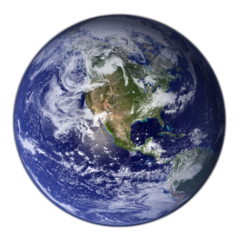
\includegraphics[width=1.8cm]{../../Figure/TBP/Earth.png}};
              % Text
              \node[below, shift={(0,-0.8)}] at (earth) {$m_1$};
              \node (a) at (A) {Earth};
              
              % Moon
              \node[circle, inner sep=5.5pt, fill=black!30] (MOON) at (moon) {};
              \node[inner sep=0pt] (moon_c) at (moon) {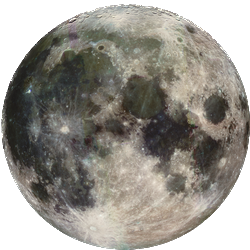
\includegraphics[width=.5cm]{../../Figure/TBP/Moon.png}};
              % Text 
              \node[below, shift={(0,-0.4)}] at (MOON) {$m_2$};
              \node (b) at (B) {Moon};
              
              % Lines
              \draw[-stealth] (a) to[bend left=30] ({\r*cos(\Phi)+1},{\r*sin(\Phi)+2});
              \draw[-stealth] (b) to[bend left=-30] (MOON);
              \draw[dashed, black] (earth) -- (MOON.center);
              
              % center of mass 0.25 from earth
              \coordinate (center) at ($(earth)!0.3!(MOON)$);
              % small circle
              \draw[fill=black] (center) circle (1.5pt) node[below, shift={(0,-0.1)}] {Center of Mass};
              
              % Calculate direction from Earth to Moon
              \pgfmathsetmacro{\xDiff}{8 - 1} % X difference between Moon and Earth
              \pgfmathsetmacro{\yDiff}{1 - 2} % Y difference between Moon and Earth
              \pgfmathsetmacro{\angle}{atan2(\yDiff,\xDiff)} % Angle of the line
              
              % Add axes at center of mass
              \draw[->, thick] (center) -- ++(\angle:2) node[above, shift={(0,0.2)}] {$x$ axis};
              \draw[->, thick] (center) -- ++(\angle+90:2) node[above] {$y$ axis};
              
              % add satellite with shift
              \coordinate (satellite) at ($(center)!0.5!(MOON)+(0,2)$);
              \node (satellite) at (satellite) {\faSpaceShuttle};
              
              % connect earth to satellite r1
              \draw[-stealth] (earth) -- (satellite) node[pos=0.3, above] {$\vb{r}_1$};   
              % connect moon to satellite r2
              \draw[-stealth] (MOON) -- (satellite) node[pos=0.5, above] {$\vb{r}_2$};
              % connect center of mass to satellite r
              \draw[-stealth] (center) -- (satellite) node[pos=0.5, above] {$\vb{r}$};
              % add line to show satellite is in between
              \node (c) at ($(satellite)+(1.5,0.5)$) {Spacecraft};
              \draw[-stealth] (c) to[bend left=30] (satellite);
            \end{tikzpicture}
          }
          \caption{CRTBP Configuration}
        \end{subfigure}%
        % \hfill
        % \hspace{-3.5cm}
        \begin{subfigure}{0.35\linewidth}
        %   \raggedleft
          \resizebox{\linewidth}{!}{%
        \begin{tikzpicture}
            % Define radius of the orbit
            \def\orbitRadius{4cm}
            
            % Draw the orbit circle with arrows
            \draw[-{Stealth[length=3mm]}, thick] (12:\orbitRadius) arc (12:170:\orbitRadius);
            \draw[-{Stealth[length=3mm]}, thick] (180:\orbitRadius) arc (180:355:\orbitRadius);
            
            % Position for Earth (center)
            \node[inner sep=0pt] (Earth) at (0,0) {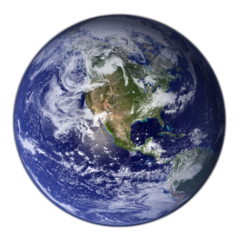
\includegraphics[width=1.8cm]{../../Figure/TBP/Earth.png}};
            \node[text=black] at (0,-1.3) {Earth};
            
            % Position for Moon (on the right side of the orbit)
            \node[inner sep=0pt] (Moon) at (0.95*\orbitRadius,0) {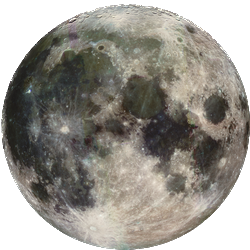
\includegraphics[width=0.6cm]{../../Figure/TBP/Moon.png}};
            \node[text=black] at (\orbitRadius,0.6) {Moon};
            
            % Lagrangian points
            \coordinate (L1) at (0.8*\orbitRadius,0);
            \coordinate (L2) at (1.2*\orbitRadius,0);
            \coordinate (L3) at (-1*\orbitRadius,0);
            \coordinate (L4) at (60:\orbitRadius);
            \coordinate (L5) at (300:\orbitRadius);
            
            % Draw Lagrangian points as red circles
            \foreach \point in {L1,L2,L3,L4,L5} {
                \fill[red] (\point) circle (0.1cm);
            }
            
            % Connect Lagrangian points with dashed lines
            \draw[dashed, blue, thick] (Earth) -- (L1);
            \draw[dashed, blue, thick] (Moon) -- (L1);
            \draw[dashed, blue, thick] (Moon) -- (L2);
            \draw[dashed, blue, thick] (Earth) -- (L3);
            \draw[dashed, blue, thick] (Earth) -- (L4);
            \draw[dashed, blue, thick] (Moon) -- (L4);
            \draw[dashed, blue, thick] (Earth) -- (L5);
            \draw[dashed, blue, thick] (Moon) -- (L5);
            
            % Labels for the Lagrangian points
            \node at ($(L1) + (0,0.5)$) {$L_1$};
            \node at ($(L2) + (0,0.5)$) {$L_2$};
            \node at ($(L3) + (0,0.5)$) {$L_3$};
            \node at ($(L4) + (0.5,0.3)$) {$L_4$};
            \node at ($(L5) + (0.5,-0.3)$) {$L_5$};
        \end{tikzpicture}
          }
        %   \raggedright
          \tiny{\caption{\tiny Lagrangian points in the Earth-Moon system}}
        \end{subfigure}
        \vspace{-0.2cm}
        % \caption{}
  \end{figure}
\end{frame}
%           \draw[-stealth] (center) -- (satellite) node[pos=0.5, above] {$\vb{r}$};
%           % add line to show satellite is in between
%           \node (c) at ($(satellite)+(1.5,0.5)$) {Satellite};
%           \draw[-stealth] (c) to[bend left=30] (satellite);
%         \end{tikzpicture}
%       }
%       \caption{CRTBP Configuration}
%     \end{subfigure}
%     \caption{Duplicated CRTBP geometric schematic (side-by-side).}
%   \end{figure}
% \end{frame}

\begin{frame}
  \frametitle{Agent Simulation in CRTBP Model}
  \begin{columns}[T]
    \begin{column}{0.5\textwidth}
      \textbf{State Representation:}
      \begin{itemize}
        \setlength{\itemsep}{-1pt}
        \item Position and velocity: $\boldsymbol{s}_t = (\delta x, \delta y, \delta \dot{x}, \delta \dot{y})$
        \item Relative to target orbit/Lagrangian point
      \end{itemize}
      
      \textbf{Action Space:}
      \begin{itemize}
        \setlength{\itemsep}{-1pt}
        \item Continuous control: $\boldsymbol{a}_t = (u_x, u_y)$
        \item Bounded thrust: $u_x, u_y \in [a_{Low}, a_{High}]$
      \end{itemize}

      \textbf{Reward Function:}
      \small
      \begin{align*}
        r(s, a) &= r_{\text{thrust}}(a) + r_{\text{reference}}(s) + r_{\text{terminal}}(s) \\[-1ex]
        r_{\text{thrust}}(a) &= -k_1 \cdot |a| \\[-1ex]
        r_{\text{reference}}(s) &= -k_2 \cdot d(s, s_{\text{reference}})
      \end{align*}
    \end{column}
    
    \begin{column}{0.5\textwidth}
      \vspace{-0.5cm}
      \begin{table}[h!]
        \scriptsize
        \centering
        \caption{\footnotesize Nondimensionalized spacecraft thrust capabilities}
        \label{tab:camparison}
    
        \setlength{\tabcolsep}{4pt}
        \renewcommand{\arraystretch}{1.1}
        \resizebox{.95\linewidth}{!}{%
        \begin{tabular}{|l|l|l|l|}
        \hline
        \textbf{Abbrv.} & \textbf{Spacecraft} & \textbf{$f_{\text{max}}$} & \textbf{$F_{\text{max}}$} \\ \hline
        DS1 & Deep Space 1 & $6.94 \cdot 10^{-2}$ & 92.0 mN \\ \hline
        Psyche & Psyche & $4.16 \cdot 10^{-2}$ & 279.3 mN \\ \hline
        Dawn & Dawn  & $2.74 \cdot 10^{-2}$ & 91.0 mN \\ \hline
        LIC & Lunar IceCube & $3.28 \cdot 10^{-2}$ & 1.25 mN \\ \hline
        H1 & Hayabusa 1 & $1.64 \cdot 10^{-2}$ & 22.8 mN \\ \hline
        H2 & Hayabusa 2 & $1.63 \cdot 10^{-2}$ & 27.0 mN \\ \hline
        s/c & Sample spacecraft & $4 \cdot 10^{-2}$ & n/a \\ \hline
        \end{tabular}
        }
      \end{table}
      \vspace{-.5cm}
      % Shift terminal reward equation 4cm to the left (over column boundary)
      \hspace*{-5cm}%
      \begin{minipage}{\dimexpr\linewidth+4cm\relax}
      \begin{align*}
        r_{\text{terminal}}(s) &= 
        \begin{cases}
          +R_{\text{goal}} & \text{if} ~ s \in S_{\text{goal}} \\[-0.5ex]
          -R_{\text{fail}} & \text{if} ~ d(s, s_{\text{ref}}) > \epsilon \\[-0.5ex]
          0 & \text{otherwise}
        \end{cases}
      \end{align*}
      \end{minipage}
    \end{column}
  \end{columns}
\end{frame}
